% Options for packages loaded elsewhere
\PassOptionsToPackage{unicode}{hyperref}
\PassOptionsToPackage{hyphens}{url}
\PassOptionsToPackage{dvipsnames,svgnames,x11names}{xcolor}
%
\documentclass[
  letterpaper,
  DIV=11,
  numbers=noendperiod]{scrartcl}

\usepackage{amsmath,amssymb}
\usepackage{iftex}
\ifPDFTeX
  \usepackage[T1]{fontenc}
  \usepackage[utf8]{inputenc}
  \usepackage{textcomp} % provide euro and other symbols
\else % if luatex or xetex
  \usepackage{unicode-math}
  \defaultfontfeatures{Scale=MatchLowercase}
  \defaultfontfeatures[\rmfamily]{Ligatures=TeX,Scale=1}
\fi
\usepackage{lmodern}
\ifPDFTeX\else  
    % xetex/luatex font selection
\fi
% Use upquote if available, for straight quotes in verbatim environments
\IfFileExists{upquote.sty}{\usepackage{upquote}}{}
\IfFileExists{microtype.sty}{% use microtype if available
  \usepackage[]{microtype}
  \UseMicrotypeSet[protrusion]{basicmath} % disable protrusion for tt fonts
}{}
\makeatletter
\@ifundefined{KOMAClassName}{% if non-KOMA class
  \IfFileExists{parskip.sty}{%
    \usepackage{parskip}
  }{% else
    \setlength{\parindent}{0pt}
    \setlength{\parskip}{6pt plus 2pt minus 1pt}}
}{% if KOMA class
  \KOMAoptions{parskip=half}}
\makeatother
\usepackage{xcolor}
\setlength{\emergencystretch}{3em} % prevent overfull lines
\setcounter{secnumdepth}{5}
% Make \paragraph and \subparagraph free-standing
\ifx\paragraph\undefined\else
  \let\oldparagraph\paragraph
  \renewcommand{\paragraph}[1]{\oldparagraph{#1}\mbox{}}
\fi
\ifx\subparagraph\undefined\else
  \let\oldsubparagraph\subparagraph
  \renewcommand{\subparagraph}[1]{\oldsubparagraph{#1}\mbox{}}
\fi

\usepackage{color}
\usepackage{fancyvrb}
\newcommand{\VerbBar}{|}
\newcommand{\VERB}{\Verb[commandchars=\\\{\}]}
\DefineVerbatimEnvironment{Highlighting}{Verbatim}{commandchars=\\\{\}}
% Add ',fontsize=\small' for more characters per line
\usepackage{framed}
\definecolor{shadecolor}{RGB}{243,245,246}
\newenvironment{Shaded}{\begin{snugshade}}{\end{snugshade}}
\newcommand{\AlertTok}[1]{\textcolor[rgb]{1.00,0.00,0.00}{\textbf{#1}}}
\newcommand{\AnnotationTok}[1]{\textcolor[rgb]{0.38,0.63,0.69}{\textbf{\textit{#1}}}}
\newcommand{\AttributeTok}[1]{\textcolor[rgb]{0.49,0.56,0.16}{#1}}
\newcommand{\BaseNTok}[1]{\textcolor[rgb]{0.25,0.63,0.44}{#1}}
\newcommand{\BuiltInTok}[1]{\textcolor[rgb]{0.00,0.50,0.00}{#1}}
\newcommand{\CharTok}[1]{\textcolor[rgb]{0.25,0.44,0.63}{#1}}
\newcommand{\CommentTok}[1]{\textcolor[rgb]{0.38,0.63,0.69}{\textit{#1}}}
\newcommand{\CommentVarTok}[1]{\textcolor[rgb]{0.38,0.63,0.69}{\textbf{\textit{#1}}}}
\newcommand{\ConstantTok}[1]{\textcolor[rgb]{0.53,0.00,0.00}{#1}}
\newcommand{\ControlFlowTok}[1]{\textcolor[rgb]{0.00,0.44,0.13}{\textbf{#1}}}
\newcommand{\DataTypeTok}[1]{\textcolor[rgb]{0.56,0.13,0.00}{#1}}
\newcommand{\DecValTok}[1]{\textcolor[rgb]{0.25,0.63,0.44}{#1}}
\newcommand{\DocumentationTok}[1]{\textcolor[rgb]{0.73,0.13,0.13}{\textit{#1}}}
\newcommand{\ErrorTok}[1]{\textcolor[rgb]{1.00,0.00,0.00}{\textbf{#1}}}
\newcommand{\ExtensionTok}[1]{\textcolor[rgb]{0.00,0.44,0.13}{#1}}
\newcommand{\FloatTok}[1]{\textcolor[rgb]{0.25,0.63,0.44}{#1}}
\newcommand{\FunctionTok}[1]{\textcolor[rgb]{0.02,0.16,0.49}{#1}}
\newcommand{\ImportTok}[1]{\textcolor[rgb]{0.00,0.50,0.00}{\textbf{#1}}}
\newcommand{\InformationTok}[1]{\textcolor[rgb]{0.38,0.63,0.69}{\textbf{\textit{#1}}}}
\newcommand{\KeywordTok}[1]{\textcolor[rgb]{0.00,0.44,0.13}{\textbf{#1}}}
\newcommand{\NormalTok}[1]{\textcolor[rgb]{0.00,0.44,0.13}{#1}}
\newcommand{\OperatorTok}[1]{\textcolor[rgb]{0.40,0.40,0.40}{#1}}
\newcommand{\OtherTok}[1]{\textcolor[rgb]{0.00,0.44,0.13}{#1}}
\newcommand{\PreprocessorTok}[1]{\textcolor[rgb]{0.74,0.48,0.00}{#1}}
\newcommand{\RegionMarkerTok}[1]{\textcolor[rgb]{0.00,0.44,0.13}{#1}}
\newcommand{\SpecialCharTok}[1]{\textcolor[rgb]{0.25,0.44,0.63}{#1}}
\newcommand{\SpecialStringTok}[1]{\textcolor[rgb]{0.73,0.40,0.53}{#1}}
\newcommand{\StringTok}[1]{\textcolor[rgb]{0.25,0.44,0.63}{#1}}
\newcommand{\VariableTok}[1]{\textcolor[rgb]{0.10,0.09,0.49}{#1}}
\newcommand{\VerbatimStringTok}[1]{\textcolor[rgb]{0.25,0.44,0.63}{#1}}
\newcommand{\WarningTok}[1]{\textcolor[rgb]{0.38,0.63,0.69}{\textbf{\textit{#1}}}}

\providecommand{\tightlist}{%
  \setlength{\itemsep}{0pt}\setlength{\parskip}{0pt}}\usepackage{longtable,booktabs,array}
\usepackage{calc} % for calculating minipage widths
% Correct order of tables after \paragraph or \subparagraph
\usepackage{etoolbox}
\makeatletter
\patchcmd\longtable{\par}{\if@noskipsec\mbox{}\fi\par}{}{}
\makeatother
% Allow footnotes in longtable head/foot
\IfFileExists{footnotehyper.sty}{\usepackage{footnotehyper}}{\usepackage{footnote}}
\makesavenoteenv{longtable}
\usepackage{graphicx}
\makeatletter
\def\maxwidth{\ifdim\Gin@nat@width>\linewidth\linewidth\else\Gin@nat@width\fi}
\def\maxheight{\ifdim\Gin@nat@height>\textheight\textheight\else\Gin@nat@height\fi}
\makeatother
% Scale images if necessary, so that they will not overflow the page
% margins by default, and it is still possible to overwrite the defaults
% using explicit options in \includegraphics[width, height, ...]{}
\setkeys{Gin}{width=\maxwidth,height=\maxheight,keepaspectratio}
% Set default figure placement to htbp
\makeatletter
\def\fps@figure{htbp}
\makeatother

\usepackage{booktabs}
\usepackage{longtable}
\usepackage{array}
\usepackage{multirow}
\usepackage{wrapfig}
\usepackage{float}
\usepackage{colortbl}
\usepackage{pdflscape}
\usepackage{tabu}
\usepackage{threeparttable}
\usepackage{threeparttablex}
\usepackage[normalem]{ulem}
\usepackage{makecell}
\usepackage{xcolor}
\KOMAoption{captions}{tableheading}
\makeatletter
\makeatother
\makeatletter
\makeatother
\makeatletter
\@ifpackageloaded{caption}{}{\usepackage{caption}}
\AtBeginDocument{%
\ifdefined\contentsname
  \renewcommand*\contentsname{Table of contents}
\else
  \newcommand\contentsname{Table of contents}
\fi
\ifdefined\listfigurename
  \renewcommand*\listfigurename{List of Figures}
\else
  \newcommand\listfigurename{List of Figures}
\fi
\ifdefined\listtablename
  \renewcommand*\listtablename{List of Tables}
\else
  \newcommand\listtablename{List of Tables}
\fi
\ifdefined\figurename
  \renewcommand*\figurename{Figure}
\else
  \newcommand\figurename{Figure}
\fi
\ifdefined\tablename
  \renewcommand*\tablename{Table}
\else
  \newcommand\tablename{Table}
\fi
}
\@ifpackageloaded{float}{}{\usepackage{float}}
\floatstyle{ruled}
\@ifundefined{c@chapter}{\newfloat{codelisting}{h}{lop}}{\newfloat{codelisting}{h}{lop}[chapter]}
\floatname{codelisting}{Listing}
\newcommand*\listoflistings{\listof{codelisting}{List of Listings}}
\makeatother
\makeatletter
\@ifpackageloaded{caption}{}{\usepackage{caption}}
\@ifpackageloaded{subcaption}{}{\usepackage{subcaption}}
\makeatother
\makeatletter
\makeatother
\ifLuaTeX
  \usepackage{selnolig}  % disable illegal ligatures
\fi
\IfFileExists{bookmark.sty}{\usepackage{bookmark}}{\usepackage{hyperref}}
\IfFileExists{xurl.sty}{\usepackage{xurl}}{} % add URL line breaks if available
\urlstyle{same} % disable monospaced font for URLs
\hypersetup{
  pdftitle={Quantifying degradation in synthesized sounds},
  colorlinks=true,
  linkcolor={blue},
  filecolor={Maroon},
  citecolor={Blue},
  urlcolor={Blue},
  pdfcreator={LaTeX via pandoc}}

\title{Quantifying degradation in synthesized sounds}
\usepackage{etoolbox}
\makeatletter
\providecommand{\subtitle}[1]{% add subtitle to \maketitle
  \apptocmd{\@title}{\par {\large #1 \par}}{}{}
}
\makeatother
\subtitle{baRulho:quantifying habitat-induced degradation of (animal)
acoustic signals}
\author{}
\date{2024-05-08}

\begin{document}
\maketitle
\renewcommand*\contentsname{Table of contents}
{
\hypersetup{linkcolor=}
\setcounter{tocdepth}{3}
\tableofcontents
}
\hypertarget{load-package}{%
\subsection{Load package}\label{load-package}}

\begin{Shaded}
\begin{Highlighting}[numbers=left,,]
\FunctionTok{library}\NormalTok{(baRulho)}
\FunctionTok{library}\NormalTok{(warbleR)}
\FunctionTok{library}\NormalTok{(ggplot2)}
\FunctionTok{library}\NormalTok{(cowplot)}
\FunctionTok{library}\NormalTok{(grid)}
\end{Highlighting}
\end{Shaded}

\hypertarget{synthetize-sounds}{%
\subsection{Synthetize sounds}\label{synthetize-sounds}}

Create synthesized sounds to be used for making the master sound file
for playback experiments:

\begin{Shaded}
\begin{Highlighting}[numbers=left,,]
\NormalTok{synth\_data }\OtherTok{\textless{}{-}}
    \FunctionTok{synth\_sounds}\NormalTok{(}
        \AttributeTok{replicates =} \DecValTok{3}\NormalTok{, }\CommentTok{\# number of replicates for each unique combination of varying features}
        \AttributeTok{frequencies =} \FunctionTok{seq}\NormalTok{(}\FloatTok{0.5}\NormalTok{, }\DecValTok{10}\NormalTok{, }\AttributeTok{length.out =} \DecValTok{20}\NormalTok{),}
        \AttributeTok{durations =} \FunctionTok{c}\NormalTok{(}\FloatTok{0.2}\NormalTok{, }\FloatTok{0.1}\NormalTok{),}
        \AttributeTok{am =} \ConstantTok{TRUE}\NormalTok{, }\CommentTok{\# amplitude modulation}
        \AttributeTok{fm =} \ConstantTok{TRUE}\NormalTok{, }\CommentTok{\# frequency modulation}
        \AttributeTok{sig2 =} \FloatTok{0.8}\NormalTok{, }\CommentTok{\# frequency modulation parameter}
        \AttributeTok{shuffle =} \ConstantTok{TRUE} \CommentTok{\# randomize the position of sounds }
\NormalTok{    )}
\end{Highlighting}
\end{Shaded}

The output is of class data frame and
\href{https://marce10.github.io/warbleR/reference/selection_table.html}{extended
selection table} (\href{https://marce10.github.io/warbleR}{warbleR}
package format, here printed as a data frame):

\begin{Shaded}
\begin{Highlighting}[numbers=left,,]
\FunctionTok{head}\NormalTok{(synth\_data, }\DecValTok{10}\NormalTok{)}
\end{Highlighting}
\end{Shaded}

\begin{landscape}
\begin{longtable*}[t]{lrrrrrlrlllrl}
\toprule
sound.files & selec & start & end & bottom.freq & top.freq & frequency & duration & frequency.modulation & amplitude.modulation & treatment & replicate & sound.id\\
\midrule
synthetic\_sound\_68 & 1 & 0.05 & 0.25 & 7.000 & 11.000 & 9 & 0.2 & fm & am & dur:0.2;freq:9;fm;am & 1 & dur:0.2;freq:9;fm;am\_1\\
synthetic\_sound\_70 & 1 & 0.05 & 0.25 & 1.990 & 6.023 & 4 & 0.2 & fm & am & dur:0.2;freq:4;fm;am & 1 & dur:0.2;freq:4;fm;am\_1\\
synthetic\_sound\_72 & 1 & 0.05 & 0.25 & 0.020 & 3.000 & 1 & 0.2 & fm & am & dur:0.2;freq:1;fm;am & 1 & dur:0.2;freq:1;fm;am\_1\\
synthetic\_sound\_119 & 1 & 0.05 & 0.25 & 4.984 & 9.009 & 7 & 0.2 & fm & am & dur:0.2;freq:7;fm;am & 1 & dur:0.2;freq:7;fm;am\_1\\
synthetic\_sound\_78 & 1 & 0.05 & 0.25 & 7.450 & 11.500 & 9.5 & 0.2 & fm & am & dur:0.2;freq:9.5;fm;am & 1 & dur:0.2;freq:9.5;fm;am\_1\\
\addlinespace
synthetic\_sound\_120 & 1 & 0.05 & 0.25 & 2.486 & 6.688 & 4.5 & 0.2 & fm & am & dur:0.2;freq:4.5;fm;am & 1 & dur:0.2;freq:4.5;fm;am\_1\\
synthetic\_sound\_86 & 1 & 0.05 & 0.25 & 0.784 & 5.000 & 3 & 0.2 & fm & am & dur:0.2;freq:3;fm;am & 1 & dur:0.2;freq:3;fm;am\_1\\
synthetic\_sound\_78 & 2 & 0.05 & 0.25 & 7.450 & 11.500 & 9.5 & 0.2 & fm & am & dur:0.2;freq:9.5;fm;am & 2 & dur:0.2;freq:9.5;fm;am\_2\\
synthetic\_sound\_33 & 1 & 0.05 & 0.25 & 0.100 & 4.000 & 2 & 0.2 & fm & am & dur:0.2;freq:2;fm;am & 1 & dur:0.2;freq:2;fm;am\_1\\
synthetic\_sound\_93 & 1 & 0.05 & 0.25 & 4.343 & 8.500 & 6.5 & 0.2 & fm & am & dur:0.2;freq:6.5;fm;am & 1 & dur:0.2;freq:6.5;fm;am\_1\\
\bottomrule
\end{longtable*}
\end{landscape}

\hypertarget{create-master-sound-file}{%
\section{Create master sound file}\label{create-master-sound-file}}

This step puts all sounds together into a single sound file:

\begin{Shaded}
\begin{Highlighting}[numbers=left,,]
\NormalTok{master\_annotations }\OtherTok{\textless{}{-}} \FunctionTok{master\_sound\_file}\NormalTok{(}\AttributeTok{X =}\NormalTok{ synth\_data, }\CommentTok{\# synthesized sound data}
                  \AttributeTok{file.name =} \StringTok{"master"}\NormalTok{, }\CommentTok{\# name of the sound file}
                  \AttributeTok{gap.duration =} \FloatTok{0.2}\NormalTok{) }\CommentTok{\# duration of silence in between sounds}
\end{Highlighting}
\end{Shaded}

The output file is saved in the current working directory (can be
modified using argument `path'). A similar file was used for the
playback experiments detailed in the paper. The following section shows
how to access the test (re-recorded) files.

These are the annotations for the sounds in the master sound files:

\begin{Shaded}
\begin{Highlighting}[numbers=left,,]
\FunctionTok{head}\NormalTok{(master\_annotations)}
\end{Highlighting}
\end{Shaded}

\begin{landscape}
\begin{longtable*}[t]{lrrrrrl}
\toprule
sound.files & selec & start & end & bottom.freq & top.freq & sound.id\\
\midrule
master.wav & 1 & 1.000000 & 2.000000 & 1.333333 & 2.666667 & start\_marker\\
master.wav & 2 & 2.050000 & 2.250023 & 7.875000 & 8.805000 & dur:0.2;freq:9;fm;am\_1\\
master.wav & 3 & 2.300023 & 2.500045 & 3.208000 & 4.069000 & dur:0.2;freq:4;fm;am\_1\\
master.wav & 4 & 2.550045 & 2.750068 & 0.422000 & 1.223000 & dur:0.2;freq:1;fm;am\_1\\
master.wav & 5 & 2.800068 & 3.000091 & 6.905000 & 7.917000 & dur:0.2;freq:7;fm;am\_1\\
\addlinespace
master.wav & 6 & 3.050091 & 3.250113 & 8.417000 & 9.416000 & dur:0.2;freq:9.5;fm;am\_1\\
master.wav & 7 & 3.300113 & 3.500136 & 4.171000 & 4.839000 & dur:0.2;freq:4.5;fm;am\_1\\
master.wav & 8 & 3.550136 & 3.750159 & 2.097000 & 2.961000 & dur:0.2;freq:3;fm;am\_1\\
master.wav & 9 & 3.800159 & 4.000181 & 9.181000 & 10.033000 & dur:0.2;freq:9.5;fm;am\_2\\
master.wav & 10 & 4.050181 & 4.250204 & 1.849000 & 2.506000 & dur:0.2;freq:2;fm;am\_1\\
\bottomrule
\end{longtable*}
\end{landscape}

\hypertarget{download-data}{%
\subsection{Download data}\label{download-data}}

This code downloads the test files. The files were re-recorded during a
transmission experiment at 10, 30, 65 and 100 m:

\begin{Shaded}
\begin{Highlighting}[numbers=left,,]
\NormalTok{path\_to\_files }\OtherTok{\textless{}{-}} \StringTok{"PATH\_TO\_FILES"}  \CommentTok{\# add folder path to keep master and test files}

\CommentTok{\# directory path where supplementary files have been saved}

\FunctionTok{options}\NormalTok{(}\AttributeTok{sound.files.path =}\NormalTok{ path\_to\_files)}

\FunctionTok{download.file}\NormalTok{(}\StringTok{"https://figshare.com/ndownloader/files/41905809"}\NormalTok{, }\AttributeTok{destfile =} \FunctionTok{file.path}\NormalTok{(path\_to\_files,}
    \StringTok{"degrad\_exp\_files.zip"}\NormalTok{))}

\FunctionTok{unzip}\NormalTok{(}\FunctionTok{file.path}\NormalTok{(path\_to\_files, }\StringTok{"degrad\_exp\_files.zip"}\NormalTok{), }\AttributeTok{exdir =} \FunctionTok{file.path}\NormalTok{(path\_to\_files))}
\end{Highlighting}
\end{Shaded}

\hypertarget{find-markers}{%
\section{Find markers}\label{find-markers}}

The code below finds the position of the start and end markers in the
test files:

\begin{Shaded}
\begin{Highlighting}[numbers=left,,]
\CommentTok{\# directory path where supplementary files have been saved}
\FunctionTok{options}\NormalTok{(}\AttributeTok{sound.files.path =}\NormalTok{ path\_to\_files)}

\NormalTok{markers\_in\_tests }\OtherTok{\textless{}{-}} \FunctionTok{find\_markers}\NormalTok{(}\AttributeTok{X =}\NormalTok{ master\_annotations)  }\CommentTok{\# annotations of sounds in master file}

\FunctionTok{head}\NormalTok{(markers\_in\_tests)}
\end{Highlighting}
\end{Shaded}

running cross-correlation (step 1 out of 2): running peak detection
(step 2 out of 2): ::: \{.cell-output-display\}

\begin{landscape}
\begin{longtable*}[t]{lrrrrlr}
\toprule
sound.files & selec & start & end & scores & marker & time.mismatch\\
\midrule
trnsc1\_100m\_closed.wav & 1 & 6.049203 & 7.049203 & 0.2228059 & start\_marker & 0.0300544\\
trnsc1\_100m\_closed.wav & 2 & 257.700686 & 258.700686 & 0.2727442 & end\_marker & NA\\
trnsc1\_100m\_open.wav & 3 & 29.502300 & 30.502300 & 0.7150524 & start\_marker & 0.0131017\\
trnsc1\_100m\_open.wav & 4 & 281.136830 & 282.136830 & 0.6083450 & end\_marker & NA\\
trnsc1\_10m\_closed.wav & 5 & 39.452253 & 40.452253 & 0.7046298 & start\_marker & 0.0114997\\
\addlinespace
trnsc1\_10m\_closed.wav & 6 & 291.085182 & 292.085182 & 0.8364759 & end\_marker & NA\\
trnsc1\_10m\_open.wav & 7 & 30.083747 & 31.083747 & 0.7667911 & start\_marker & 0.0208117\\
trnsc1\_10m\_open.wav & 8 & 281.725987 & 282.725987 & 0.8284335 & end\_marker & NA\\
trnsc1\_1m\_open.wav & 9 & 100.116084 & 101.116084 & 0.8674470 & start\_marker & 0.0097773\\
trnsc1\_1m\_open.wav & 10 & 351.747290 & 352.747290 & 0.8857788 & end\_marker & NA\\
\bottomrule
\end{longtable*}
\end{landscape}

:::

The column `time.mismatch' compares the time difference between the two
templates on test-files against that in the master sound file. In a
perfect marker detection the value must be 0, meaning that the time in
between markers in the master and test files is exactly the same. In
this case the average mismatch is of 14 ms and the highest of 32 ms:

\begin{Shaded}
\begin{Highlighting}[numbers=left,,]
\CommentTok{\# average mismatch}
\FunctionTok{mean}\NormalTok{(markers\_in\_tests}\SpecialCharTok{$}\NormalTok{time.mismatch, }\AttributeTok{na.rm =} \ConstantTok{TRUE}\NormalTok{)}
\end{Highlighting}
\end{Shaded}

\begin{verbatim}
[1] 0.01438455
\end{verbatim}

\begin{Shaded}
\begin{Highlighting}[numbers=left,,]
\CommentTok{\# maximum mismatch}
\FunctionTok{max}\NormalTok{(markers\_in\_tests}\SpecialCharTok{$}\NormalTok{time.mismatch, }\AttributeTok{na.rm =} \ConstantTok{TRUE}\NormalTok{)}
\end{Highlighting}
\end{Shaded}

\begin{verbatim}
[1] 0.03171009
\end{verbatim}

Modifying detection parameters as spectrogram type (`type' argument),
time window overlap (`ovlp' argument) and hop size (`hop.size' argument)
can be adjusted in order to improve precision. Note that for aligning
all other sounds only the marker with the highest correlation will be
used. Therefore the time mismatch is likely to be lower in the aligned
test sounds.

\hypertarget{align-sounds}{%
\section{Align sounds}\label{align-sounds}}

Once we know the position of markers we can compute the position for all
other sounds in the test files (i.e.~align):

\begin{Shaded}
\begin{Highlighting}[numbers=left,,]
\NormalTok{aligned\_tests }\OtherTok{\textless{}{-}}
    \FunctionTok{align\_test\_files}\NormalTok{(}\AttributeTok{X =}\NormalTok{ master\_annotations, }\CommentTok{\# annotations of sounds in master file}
                     \AttributeTok{Y =}\NormalTok{ markers\_in\_tests) }\CommentTok{\# position of markers in test files}
                    

\FunctionTok{head}\NormalTok{(aligned\_tests)}
\end{Highlighting}
\end{Shaded}

\begin{landscape}
\begin{longtable*}[t]{lrrrrrll}
\toprule
sound.files & selec & start & end & bottom.freq & top.freq & sound.id & marker\\
\midrule
trnsc1\_100m\_closed.wav & 1 & 6.060315 & 7.060315 & 1.333333 & 2.666667 & start\_marker & end\_marker\\
trnsc1\_100m\_closed.wav & 2 & 7.110315 & 7.310338 & 7.875000 & 8.805000 & dur:0.2;freq:9;fm;am\_1 & end\_marker\\
trnsc1\_100m\_closed.wav & 3 & 7.360338 & 7.560361 & 3.208000 & 4.069000 & dur:0.2;freq:4;fm;am\_1 & end\_marker\\
trnsc1\_100m\_closed.wav & 4 & 7.610361 & 7.810383 & 0.422000 & 1.223000 & dur:0.2;freq:1;fm;am\_1 & end\_marker\\
trnsc1\_100m\_closed.wav & 5 & 7.860383 & 8.060406 & 6.905000 & 7.917000 & dur:0.2;freq:7;fm;am\_1 & end\_marker\\
\addlinespace
trnsc1\_100m\_closed.wav & 6 & 8.110406 & 8.310429 & 8.417000 & 9.416000 & dur:0.2;freq:9.5;fm;am\_1 & end\_marker\\
trnsc1\_100m\_closed.wav & 7 & 8.360429 & 8.560451 & 4.171000 & 4.839000 & dur:0.2;freq:4.5;fm;am\_1 & end\_marker\\
trnsc1\_100m\_closed.wav & 8 & 8.610451 & 8.810474 & 2.097000 & 2.961000 & dur:0.2;freq:3;fm;am\_1 & end\_marker\\
trnsc1\_100m\_closed.wav & 9 & 8.860474 & 9.060497 & 9.181000 & 10.033000 & dur:0.2;freq:9.5;fm;am\_2 & end\_marker\\
trnsc1\_100m\_closed.wav & 10 & 9.110497 & 9.310519 & 1.849000 & 2.506000 & dur:0.2;freq:2;fm;am\_1 & end\_marker\\
\bottomrule
\end{longtable*}
\end{landscape}

Alignments can be manually adjusted with the function
\texttt{manual\_realign()}. he function generates a multipanel graph
with the spectrogram of the master sound file in top of that from test
sound files, highlighting the position of correspondent test sounds on
both in order to simplify assessing and adjusting their alignment.
Spectrograms include the first few seconds of the sound files
(controlled by `duration') which is usually enough to tell the precision
of the alignment. The lower spectrogram shows a series of `buttons' that
users can click on to control if the test sound file spectrogram (low
panel) needs to be moved to the left (``\textless{}'') or right
(``\textgreater{}''). Users can also reset the spectrogram to its
original position (`reset'), move on to the next sound file in `X' (test
sound file annotations) or stop the process (stop button). The function
returns an object similar to the input object `X' in which the start and
end of the sounds have been adjusted:

\begin{Shaded}
\begin{Highlighting}[numbers=left,,]
\NormalTok{realigned\_tests }\OtherTok{\textless{}{-}} \FunctionTok{manual\_realign}\NormalTok{(}\AttributeTok{X =}\NormalTok{ aligned\_tests, }\AttributeTok{Y =}\NormalTok{ master\_annotations,}
    \AttributeTok{marker =} \StringTok{"end\_marker"}\NormalTok{, }\AttributeTok{flim =} \FunctionTok{c}\NormalTok{(}\DecValTok{0}\NormalTok{, }\DecValTok{6}\NormalTok{))}
\end{Highlighting}
\end{Shaded}

\begin{figure}

{\centering \includegraphics{../output/manual_realign.gif}

}

\caption{manual\_realign}

\end{figure}

This plot shows the aligned re-recorded sounds for transect 1:

\begin{figure}

{\centering 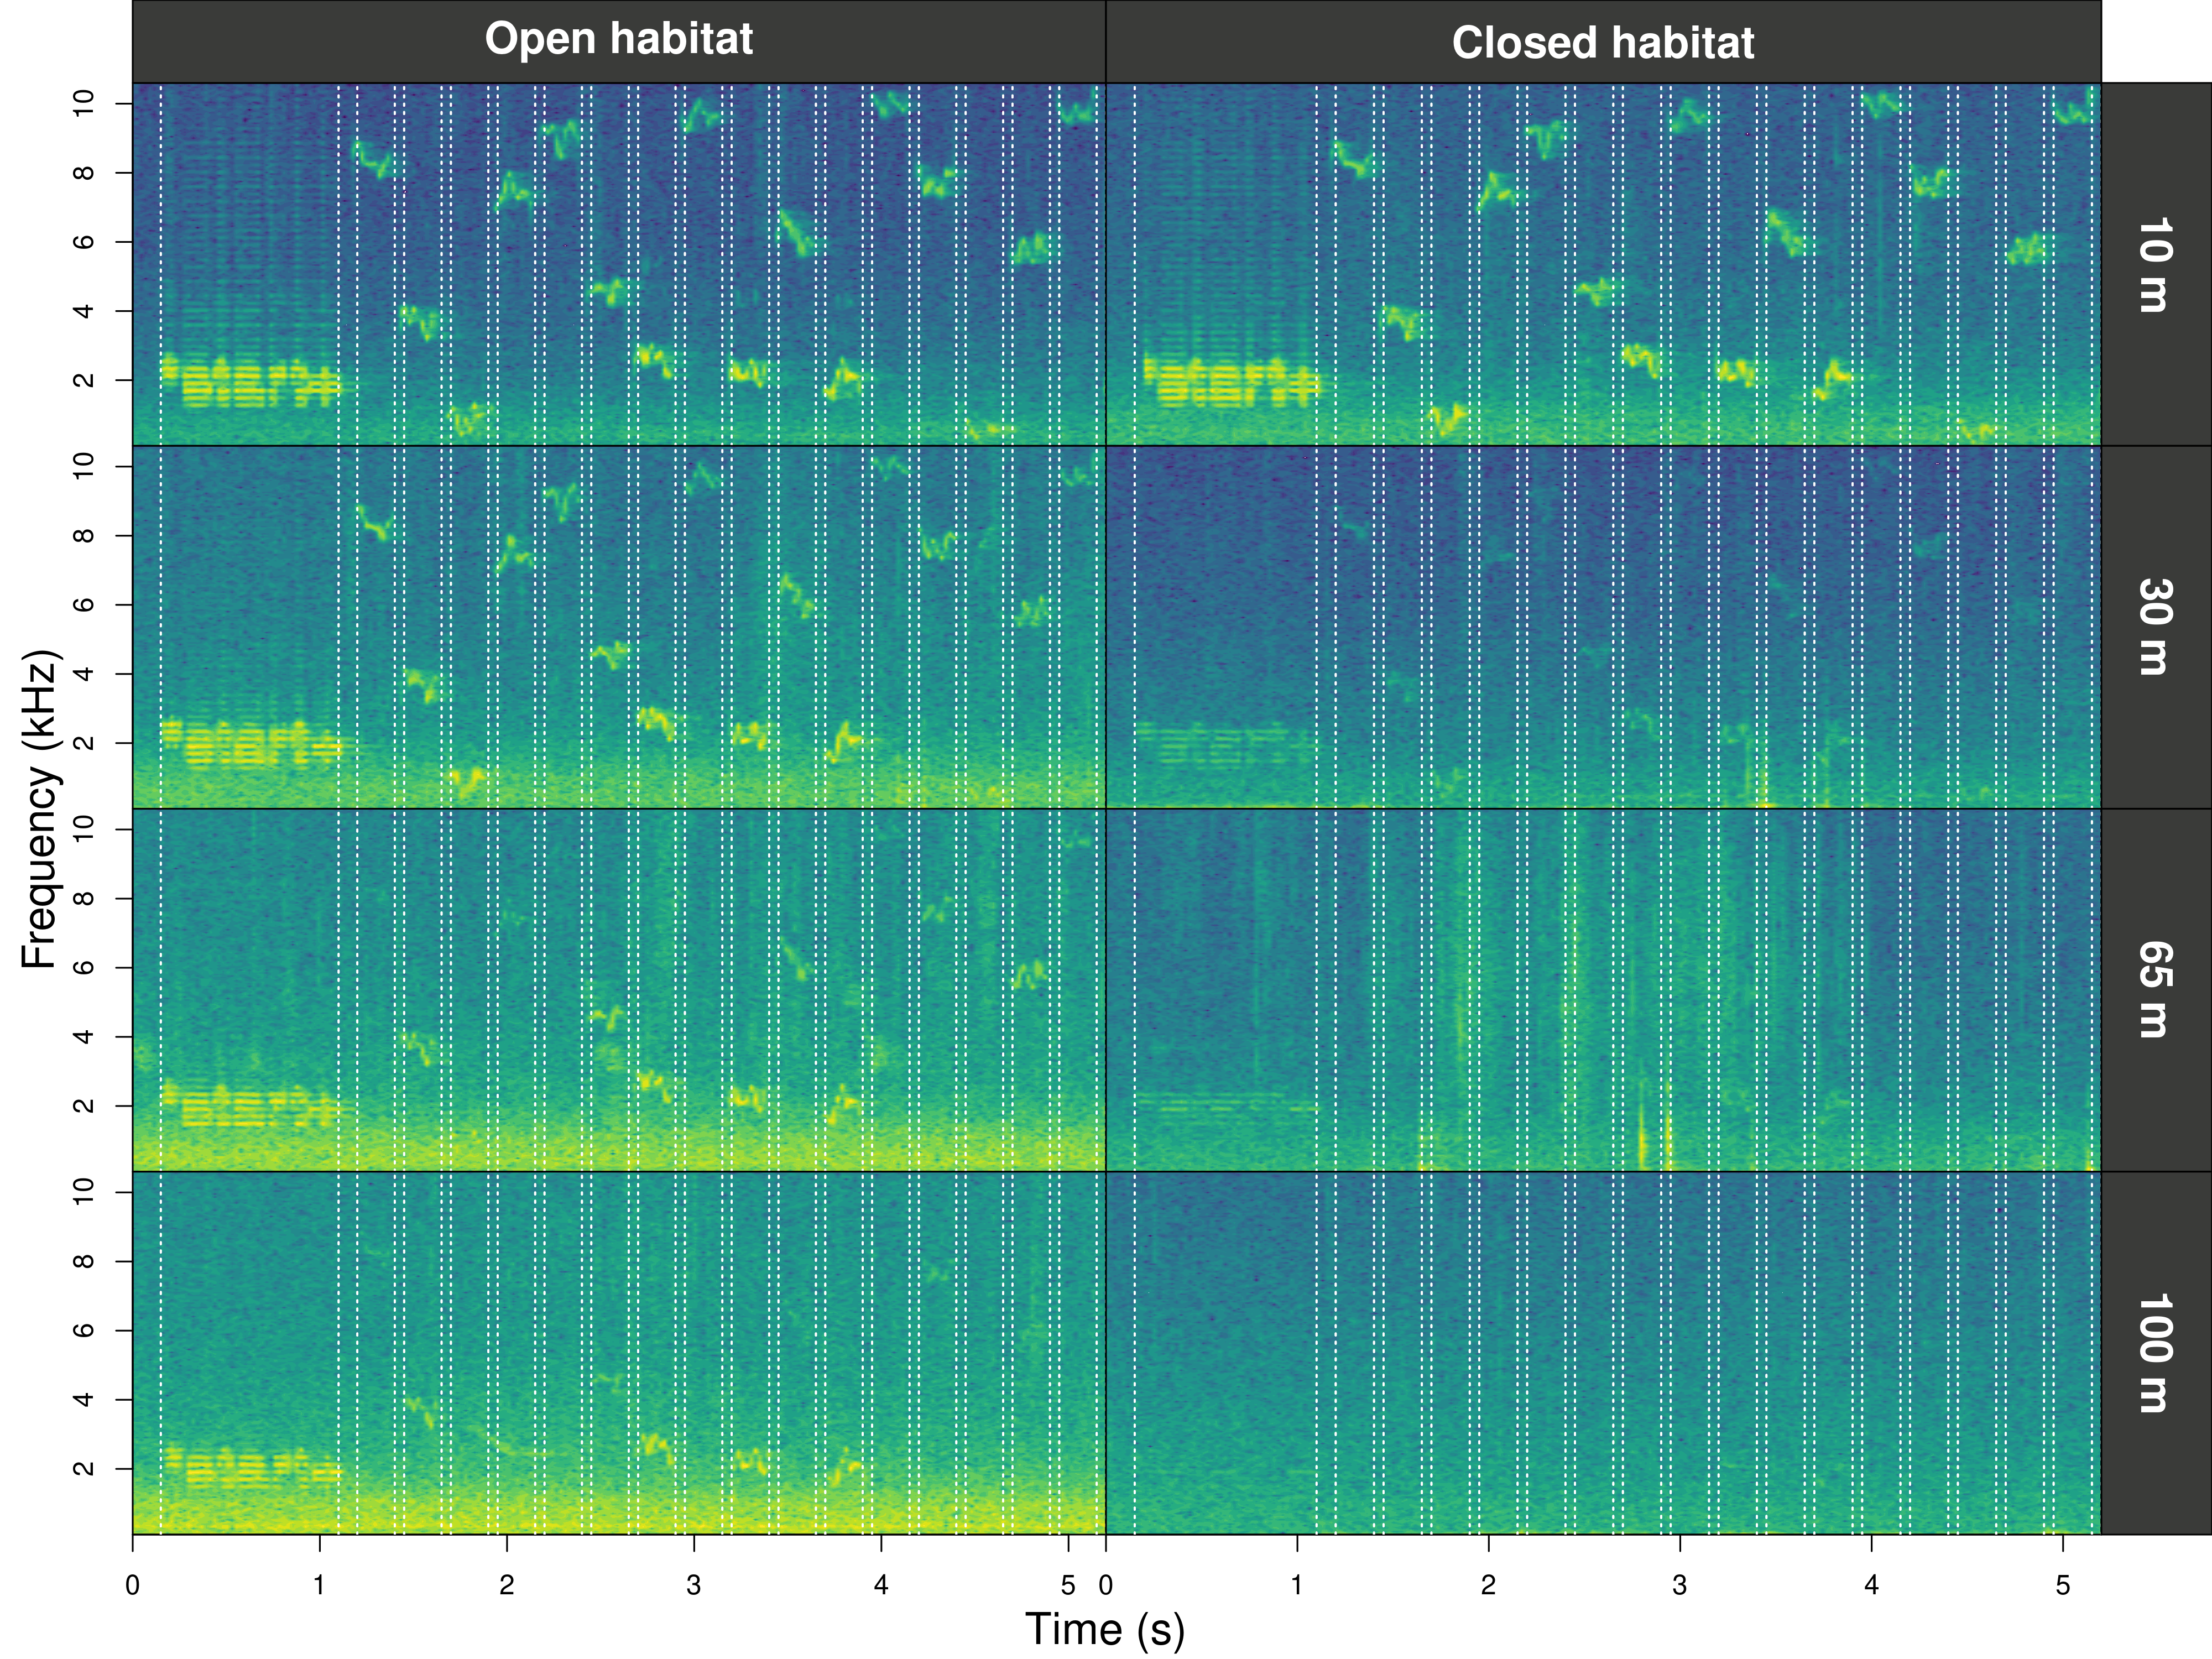
\includegraphics{../output/spectrograms_by_habitat_and_distance_transect2.png}

}

\caption{Fourier spectrograms of test recordings from the third
experimental transect in the two habitat types (columns) and four
distances (rows). The dotted vertical lines highlight the detected
position of sounds computed by the functions find\_markers and
align\_test\_files.}

\end{figure}

Similar images can be generated for each test sound file with the
function `plot\_align\_sounds()'.

\hypertarget{measuring-degradation}{%
\section{Measuring degradation}\label{measuring-degradation}}

Must degradation metrics involve comparing tests sounds that were
recorded at different distances from the speaker, to their reference,
which is typically recorded at 1m. Hence, a column indicating the
distance at which each sound was recorded is needed. In this case the
recording distance can be extracted from the sound file name:

\begin{Shaded}
\begin{Highlighting}[numbers=left,,]
\CommentTok{\# get distance}
\NormalTok{realigned\_tests}\SpecialCharTok{$}\NormalTok{distance }\OtherTok{\textless{}{-}} \FunctionTok{sapply}\NormalTok{(}\FunctionTok{strsplit}\NormalTok{(realigned\_tests}\SpecialCharTok{$}\NormalTok{sound.files,}
    \StringTok{"\_"}\NormalTok{), }\StringTok{"[["}\NormalTok{, }\DecValTok{2}\NormalTok{)}

\CommentTok{\# make it a numeric column}
\NormalTok{realigned\_tests}\SpecialCharTok{$}\NormalTok{distance }\OtherTok{\textless{}{-}} \FunctionTok{as.numeric}\NormalTok{(}\FunctionTok{gsub}\NormalTok{(}\StringTok{"m"}\NormalTok{, }\StringTok{""}\NormalTok{, realigned\_tests}\SpecialCharTok{$}\NormalTok{distance))}
\end{Highlighting}
\end{Shaded}

Once the distance is included in the annotations degradation metrics can
be obtained with few lines of code. First the function
`set\_reference\_sounds()' is used to define the reference for each test
sound:

\begin{Shaded}
\begin{Highlighting}[numbers=left,,]
\NormalTok{test\_data }\OtherTok{\textless{}{-}} \FunctionTok{set\_reference\_sounds}\NormalTok{(realigned\_tests, }\AttributeTok{method =} \DecValTok{1}\NormalTok{)}
\end{Highlighting}
\end{Shaded}

For instance the following code computes excess attenuation,
signal-to-noise ratio, blur ratio and tail-to-signal ratio:

\begin{Shaded}
\begin{Highlighting}[numbers=left,,]
\CommentTok{\# get degradation measures}
\NormalTok{degrad\_df }\OtherTok{\textless{}{-}} \FunctionTok{blur\_ratio}\NormalTok{(test\_data)}

\NormalTok{degrad\_df }\OtherTok{\textless{}{-}} \FunctionTok{excess\_attenuation}\NormalTok{(degrad\_df)}

\NormalTok{degrad\_df }\OtherTok{\textless{}{-}} \FunctionTok{signal\_to\_noise\_ratio}\NormalTok{(degrad\_df, }
                                   \AttributeTok{mar =} \FloatTok{0.1}\NormalTok{) }\CommentTok{\# mar = margin to measure noise}

\NormalTok{degrad\_df }\OtherTok{\textless{}{-}} \FunctionTok{tail\_to\_signal\_ratio}\NormalTok{(degrad\_df, }\AttributeTok{mar =} \FloatTok{0.1}\NormalTok{) }\CommentTok{\# mar = margin to measure tail}

\CommentTok{\# or as a pipe}
\NormalTok{degrad\_df }\OtherTok{\textless{}{-}}\NormalTok{ test\_data }\SpecialCharTok{|\textgreater{}}
    \FunctionTok{excess\_attenuation}\NormalTok{() }\SpecialCharTok{|\textgreater{}}
    \FunctionTok{signal\_to\_noise\_ratio}\NormalTok{(}\AttributeTok{mar =} \FloatTok{0.1}\NormalTok{) }\SpecialCharTok{|\textgreater{}} \CommentTok{\# mar = margin to measure noise}
    \FunctionTok{blur\_ratio}\NormalTok{() }\SpecialCharTok{|\textgreater{}}
    \FunctionTok{tail\_to\_signal\_ratio}\NormalTok{(}\AttributeTok{mar =} \FloatTok{0.1}\NormalTok{) }\CommentTok{\# mar = margin to measure tail}

\FunctionTok{head}\NormalTok{(realigned\_tests) }\CommentTok{\# print the first 6 rows}
\end{Highlighting}
\end{Shaded}

\begin{landscape}
\begin{longtable*}[t]{lrrrrrllrlrrrr}
\toprule
sound.files & selec & start & end & bottom.freq & top.freq & sound.id & marker & distance & reference & excess.attenuation & signal.to.noise.ratio & blur.ratio & tail.to.signal.ratio\\
\midrule
trnsc1\_100m\_closed.wav & 2 & 7.110315 & 7.310338 & 7.875 & 8.805 & dur:0.2;freq:9;fm;am\_1 & end\_marker & 100 & trnsc1\_1m\_open.wav-2 & 8.999975 & 0.7685672 & 0.2920241 & -0.9995171\\
trnsc1\_100m\_closed.wav & 3 & 7.360338 & 7.560361 & 3.208 & 4.069 & dur:0.2;freq:4;fm;am\_1 & end\_marker & 100 & trnsc1\_1m\_open.wav-3 & 10.829675 & 0.6384587 & 0.2976129 & 0.1901690\\
trnsc1\_100m\_closed.wav & 4 & 7.610361 & 7.810383 & 0.422 & 1.223 & dur:0.2;freq:1;fm;am\_1 & end\_marker & 100 & trnsc1\_1m\_open.wav-4 & 26.216040 & 4.5246601 & 0.1418792 & 2.4441865\\
trnsc1\_100m\_closed.wav & 5 & 7.860383 & 8.060406 & 6.905 & 7.917 & dur:0.2;freq:7;fm;am\_1 & end\_marker & 100 & trnsc1\_1m\_open.wav-5 & 15.191104 & -1.3816010 & 0.2667528 & 0.0593048\\
trnsc1\_100m\_closed.wav & 6 & 8.110406 & 8.310429 & 8.417 & 9.416 & dur:0.2;freq:9.5;fm;am\_1 & end\_marker & 100 & trnsc1\_1m\_open.wav-6 & 6.041307 & -0.2574492 & 0.2059137 & -1.2052163\\
\addlinespace
trnsc1\_100m\_closed.wav & 7 & 8.360429 & 8.560451 & 4.171 & 4.839 & dur:0.2;freq:4.5;fm;am\_1 & end\_marker & 100 & trnsc1\_1m\_open.wav-7 & 12.278579 & -0.7122037 & 0.2213225 & 1.6697592\\
trnsc1\_1m\_open.wav & 2 & 101.161071 & 101.361094 & 7.875 & 8.805 & dur:0.2;freq:9;fm;am\_1 & end\_marker & 1 & NA & NA & 33.4608871 & NA & -44.7221579\\
trnsc1\_1m\_open.wav & 3 & 101.411094 & 101.611117 & 3.208 & 4.069 & dur:0.2;freq:4;fm;am\_1 & end\_marker & 1 & NA & NA & 34.3281762 & NA & -30.4723829\\
trnsc1\_1m\_open.wav & 4 & 101.661117 & 101.861139 & 0.422 & 1.223 & dur:0.2;freq:1;fm;am\_1 & end\_marker & 1 & NA & NA & 26.4757912 & NA & -28.0007211\\
trnsc1\_1m\_open.wav & 5 & 101.911139 & 102.111162 & 6.905 & 7.917 & dur:0.2;freq:7;fm;am\_1 & end\_marker & 1 & NA & NA & 26.5792970 & NA & -43.0454921\\
\bottomrule
\end{longtable*}
\end{landscape}

The package can also generate images to inspect the patterns of
degradation on different acoustic dimension. The function
`plot\_degradation()' produces JPEG files with a mosaic of visual
representations of sounds (spectrograms, power spectrum and amplitude
envelopes) for each test sound and correspondent reference sound

\begin{Shaded}
\begin{Highlighting}[numbers=left,,]
\FunctionTok{options}\NormalTok{(}\AttributeTok{dest.path =} \StringTok{"DIRECTORY\_TO\_SAVE\_IMAGE\_FILES"}\NormalTok{)}
\FunctionTok{plot\_degradation}\NormalTok{(}\AttributeTok{X =}\NormalTok{ test\_data)}
\end{Highlighting}
\end{Shaded}

\begin{figure}

{\centering 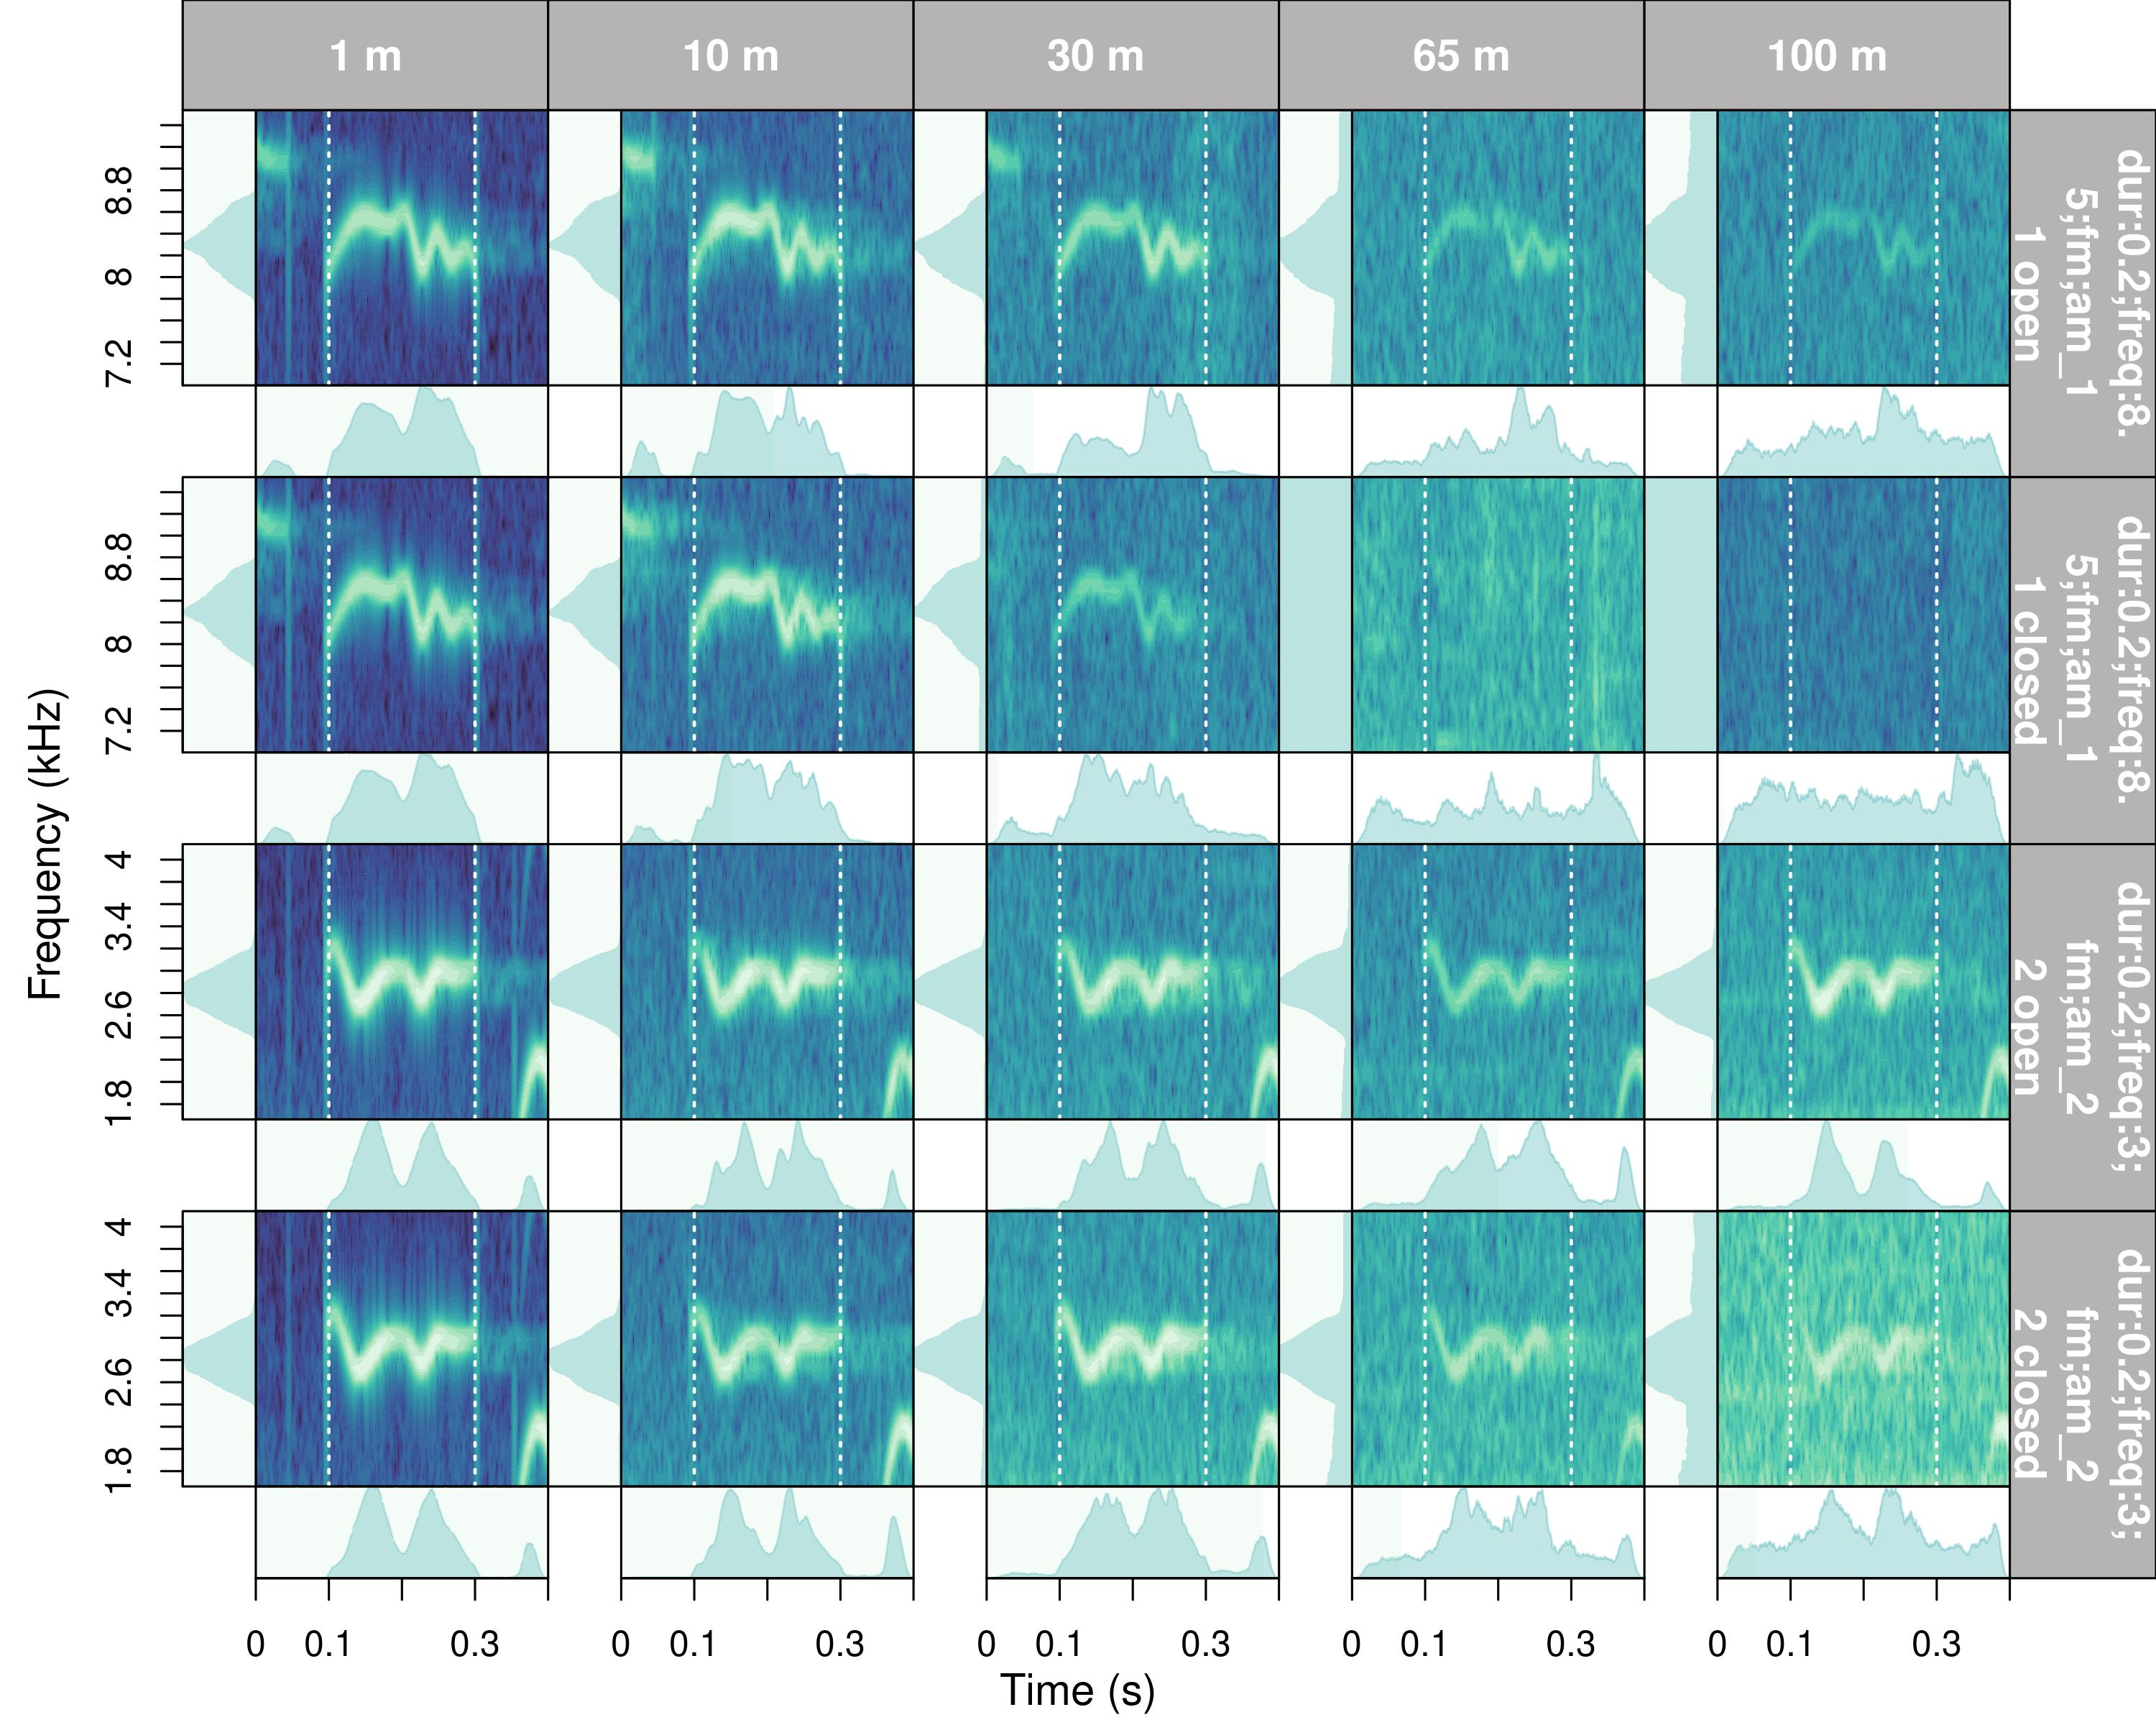
\includegraphics{plot_degradation_p1.jpeg}

}

\caption{Example of the output image files from plot\_degradation()
showing the spectrogram, amplitude envelope and power spectrum for each
test sound and its correspondent reference arranged by sound ID and
transect.}

\end{figure}

THe function \texttt{plot\_blur\_ratio()} can help explore more closely
the effects of degradation on signal structure. It generates image files
(in `jpeg' format) for each possible blur ratio estimation in the test
sound data. The image files show the spectrograms of both sounds and the
overlaid energy distribution (either amplitude envelopes or power
spectrum, see argument `type') as probability mass functions (PMF). The
output graphs highlight the mismatch between the compared distribution
which represent the estimated blur ratio returned by either
\texttt{blur\_ratio()} or \texttt{spectrum\_blur\_ratio()}.

Amplitude envelope blur ratio (or simply blur ratio):

\begin{Shaded}
\begin{Highlighting}[numbers=left,,]
\FunctionTok{plot\_blur\_ratio}\NormalTok{(}\AttributeTok{X =}\NormalTok{ test\_data, }\AttributeTok{ovlp =} \DecValTok{95}\NormalTok{, }\AttributeTok{cores =} \DecValTok{20}\NormalTok{, }\AttributeTok{dest.path =} \FunctionTok{tempdir}\NormalTok{())}
\end{Highlighting}
\end{Shaded}

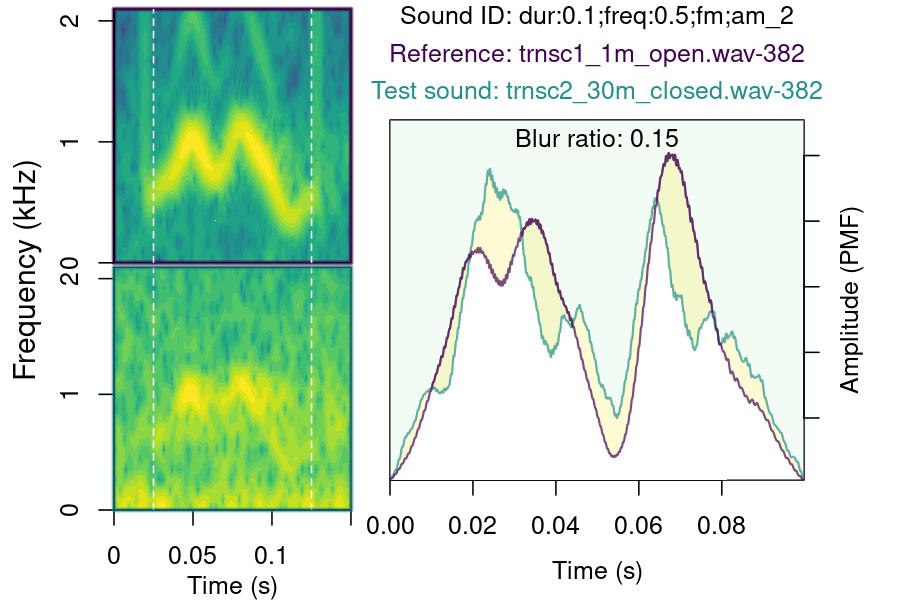
\includegraphics{blur_ratio_dur:0.1;freq:0.5;fm;am_2-trnsc1_1m_open.wav-382-trnsc2_30m_closed.wav-382.jpeg}
Power spectrum blur ratio:

\begin{Shaded}
\begin{Highlighting}[numbers=left,,]
\FunctionTok{plot\_blur\_ratio}\NormalTok{(}\AttributeTok{X =}\NormalTok{ test\_data, }\AttributeTok{type =} \StringTok{"spectrum"}\NormalTok{, }\AttributeTok{ovlp =} \DecValTok{95}\NormalTok{, }\AttributeTok{cores =} \DecValTok{20}\NormalTok{,}
    \AttributeTok{dest.path =} \FunctionTok{tempdir}\NormalTok{())}
\end{Highlighting}
\end{Shaded}

\begin{figure}

{\centering 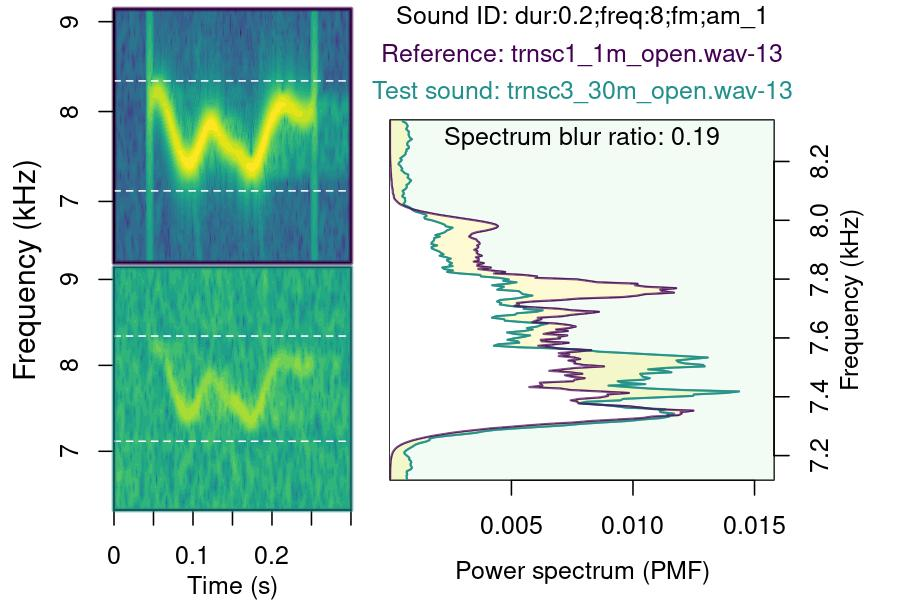
\includegraphics{spectrum_blur_ratio_dur:0.2;freq:8;fm;am_1-trnsc1_1m_open.wav-13-trnsc3_30m_open.wav-13.jpeg}

}

\caption{Example of the output image files from plot\_blur\_ratio()
(when type = `spectrum') showing the overlaid power spectrum of the test
sound and its reference, the mismatch between the two, and the
spectrograms for both}

\end{figure}

Spectrograms are shown within the frequency range of the reference sound
and also show vertical lines with the start and end of sounds.

Finally, plotting degradation metrics against distance can give us a
sense of how well each of them quantify aspects of degradation as this
is expected to increase with distance:

\begin{Shaded}
\begin{Highlighting}[numbers=left,,]
\DocumentationTok{\#\# prepare data add habitat strucvture}
\NormalTok{degrad\_df}\SpecialCharTok{$}\NormalTok{habitat.structure }\OtherTok{\textless{}{-}} \FunctionTok{ifelse}\NormalTok{(}\FunctionTok{grepl}\NormalTok{(}\StringTok{"closed"}\NormalTok{, degrad\_df}\SpecialCharTok{$}\NormalTok{sound.files),}
    \StringTok{"closed"}\NormalTok{, }\StringTok{"open"}\NormalTok{)}
\FunctionTok{names}\NormalTok{(degrad\_df)}

\CommentTok{\# select subset of 3 kHz tonal flat sounds and aggregate by}
\CommentTok{\# distance mean}
\NormalTok{agg\_degrad }\OtherTok{\textless{}{-}} \FunctionTok{aggregate}\NormalTok{(}\FunctionTok{cbind}\NormalTok{(blur.ratio, spectrum.blur.ratio, excess.attenuation,}
\NormalTok{    envelope.correlation, spectrum.correlation, cross.correlation,}
\NormalTok{    signal.to.noise.ratio, tail.to.signal.ratio) }\SpecialCharTok{\textasciitilde{}}\NormalTok{ distance }\SpecialCharTok{+}\NormalTok{ habitat.structure,}
\NormalTok{    degrad\_df[degrad\_df}\SpecialCharTok{$}\NormalTok{distance }\SpecialCharTok{\textgreater{}} \DecValTok{1} \SpecialCharTok{\&} \FunctionTok{grepl}\NormalTok{(}\StringTok{"freq:3;tonal;flat"}\NormalTok{,}
\NormalTok{        degrad\_df}\SpecialCharTok{$}\NormalTok{sound.id), ], mean)}

\CommentTok{\# and SD}
\NormalTok{agg\_degrad\_sd }\OtherTok{\textless{}{-}} \FunctionTok{aggregate}\NormalTok{(}\FunctionTok{cbind}\NormalTok{(blur.ratio, spectrum.blur.ratio,}
\NormalTok{    excess.attenuation, envelope.correlation, spectrum.correlation,}
\NormalTok{    cross.correlation, signal.to.noise.ratio, tail.to.signal.ratio) }\SpecialCharTok{\textasciitilde{}}
\NormalTok{    distance }\SpecialCharTok{+}\NormalTok{ habitat.structure, degrad\_df[degrad\_df}\SpecialCharTok{$}\NormalTok{distance }\SpecialCharTok{\textgreater{}} \DecValTok{1} \SpecialCharTok{\&}
    \FunctionTok{grepl}\NormalTok{(}\StringTok{"freq:5;tonal;flat"}\NormalTok{, degrad\_df}\SpecialCharTok{$}\NormalTok{sound.id), ], sd)}

\CommentTok{\# stack to use with ggplot2}
\NormalTok{stck\_degrad }\OtherTok{\textless{}{-}} \FunctionTok{stack}\NormalTok{(agg\_degrad)}
\NormalTok{stck\_degrad}\SpecialCharTok{$}\NormalTok{distance }\OtherTok{\textless{}{-}} \FunctionTok{as.numeric}\NormalTok{(stck\_degrad}\SpecialCharTok{$}\NormalTok{values[stck\_degrad}\SpecialCharTok{$}\NormalTok{ind }\SpecialCharTok{==}
    \StringTok{"distance"}\NormalTok{])}
\NormalTok{stck\_degrad}\SpecialCharTok{$}\NormalTok{habitat.structure }\OtherTok{\textless{}{-}}\NormalTok{ stck\_degrad}\SpecialCharTok{$}\NormalTok{values[stck\_degrad}\SpecialCharTok{$}\NormalTok{ind }\SpecialCharTok{==}
    \StringTok{"habitat.structure"}\NormalTok{]}
\NormalTok{stck\_degrad }\OtherTok{\textless{}{-}}\NormalTok{ stck\_degrad[}\SpecialCharTok{{-}}\DecValTok{1}\SpecialCharTok{:{-}}\DecValTok{16}\NormalTok{, ]}
\NormalTok{stck\_degrad\_sd }\OtherTok{\textless{}{-}} \FunctionTok{stack}\NormalTok{(agg\_degrad\_sd)[}\SpecialCharTok{{-}}\DecValTok{1}\SpecialCharTok{:{-}}\DecValTok{16}\NormalTok{, ]}
\NormalTok{stck\_degrad}\SpecialCharTok{$}\NormalTok{sd }\OtherTok{\textless{}{-}} \FunctionTok{as.numeric}\NormalTok{(stck\_degrad\_sd}\SpecialCharTok{$}\NormalTok{values)}
\NormalTok{stck\_degrad}\SpecialCharTok{$}\NormalTok{values }\OtherTok{\textless{}{-}} \FunctionTok{as.numeric}\NormalTok{(stck\_degrad}\SpecialCharTok{$}\NormalTok{values)}
\NormalTok{stck\_degrad}\SpecialCharTok{$}\NormalTok{ind }\OtherTok{\textless{}{-}} \FunctionTok{gsub}\NormalTok{(}\StringTok{"}\SpecialCharTok{\textbackslash{}\textbackslash{}}\StringTok{."}\NormalTok{, }\StringTok{" "}\NormalTok{, stck\_degrad}\SpecialCharTok{$}\NormalTok{ind)}
\NormalTok{stck\_degrad}\SpecialCharTok{$}\NormalTok{ind }\OtherTok{\textless{}{-}} \FunctionTok{gsub}\NormalTok{(}\StringTok{" to "}\NormalTok{, }\StringTok{"{-}to{-}"}\NormalTok{, stck\_degrad}\SpecialCharTok{$}\NormalTok{ind)}

\CommentTok{\# plot}
\NormalTok{gg }\OtherTok{\textless{}{-}} \FunctionTok{ggplot}\NormalTok{(}\AttributeTok{data =}\NormalTok{ stck\_degrad, }\FunctionTok{aes}\NormalTok{(}\AttributeTok{x =}\NormalTok{ distance, }\AttributeTok{y =}\NormalTok{ values, }\AttributeTok{color =}\NormalTok{ habitat.structure)) }\SpecialCharTok{+}
    \FunctionTok{geom\_point}\NormalTok{(}\AttributeTok{size =} \DecValTok{3}\NormalTok{) }\SpecialCharTok{+} \FunctionTok{geom\_errorbar}\NormalTok{(}\FunctionTok{aes}\NormalTok{(}\AttributeTok{ymin =}\NormalTok{ values }\SpecialCharTok{{-}}\NormalTok{ sd, }\AttributeTok{ymax =}\NormalTok{ values }\SpecialCharTok{+}
\NormalTok{    sd), }\AttributeTok{width =} \DecValTok{0}\NormalTok{) }\SpecialCharTok{+} \FunctionTok{geom\_line}\NormalTok{(}\FunctionTok{aes}\NormalTok{(}\AttributeTok{colour =}\NormalTok{ habitat.structure, }\AttributeTok{group =}\NormalTok{ habitat.structure)) }\SpecialCharTok{+}
    \FunctionTok{scale\_color\_viridis\_d}\NormalTok{(}\AttributeTok{alpha =} \FloatTok{0.6}\NormalTok{, }\AttributeTok{begin =} \FloatTok{0.3}\NormalTok{, }\AttributeTok{end =} \FloatTok{0.8}\NormalTok{) }\SpecialCharTok{+} \FunctionTok{facet\_wrap}\NormalTok{(}\SpecialCharTok{\textasciitilde{}}\NormalTok{ind,}
    \AttributeTok{ncol =} \DecValTok{2}\NormalTok{, }\AttributeTok{scales =} \StringTok{"free\_y"}\NormalTok{) }\SpecialCharTok{+} \FunctionTok{theme\_classic}\NormalTok{() }\SpecialCharTok{+} \FunctionTok{scale\_x\_continuous}\NormalTok{(}\AttributeTok{breaks =} \FunctionTok{unique}\NormalTok{(stck\_degrad}\SpecialCharTok{$}\NormalTok{distance),}
    \AttributeTok{labels =} \FunctionTok{unique}\NormalTok{(stck\_degrad}\SpecialCharTok{$}\NormalTok{distance)) }\SpecialCharTok{+} \FunctionTok{labs}\NormalTok{(}\AttributeTok{color =} \StringTok{"Habitat}\SpecialCharTok{\textbackslash{}n}\StringTok{structure"}\NormalTok{,}
    \AttributeTok{x =} \StringTok{"Distance (m)"}\NormalTok{, }\AttributeTok{y =} \StringTok{"Values"}\NormalTok{)}

\NormalTok{gg}
\end{Highlighting}
\end{Shaded}

\begin{figure}

{\centering 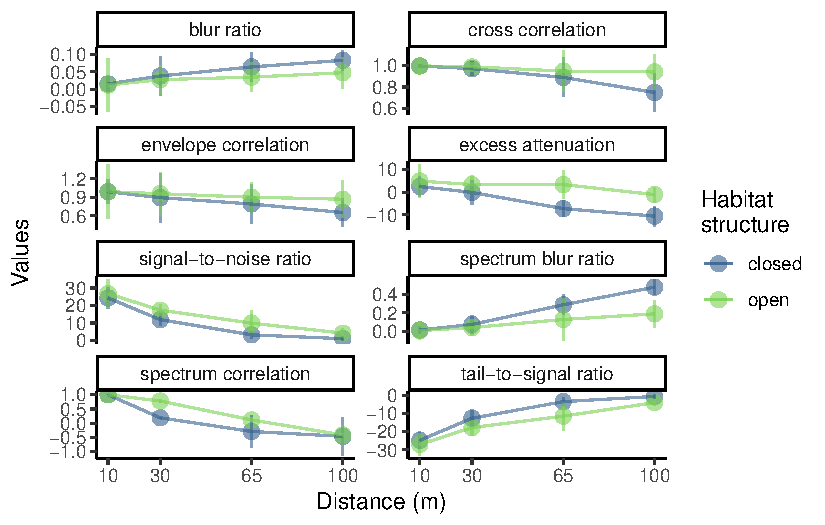
\includegraphics{Example-data-analysis-for-manuscript_files/figure-pdf/unnamed-chunk-27-1.pdf}

}

\caption{Mean degradation metrics (+/- s.d.) by distance and habitat
structure types}

\end{figure}

\begin{center}\rule{0.5\linewidth}{0.5pt}\end{center}

Session information

\begin{verbatim}
R version 4.3.3 (2024-02-29)
Platform: x86_64-pc-linux-gnu (64-bit)
Running under: Ubuntu 22.04.4 LTS

Matrix products: default
BLAS:   /usr/lib/x86_64-linux-gnu/blas/libblas.so.3.10.0 
LAPACK: /usr/lib/x86_64-linux-gnu/lapack/liblapack.so.3.10.0

locale:
 [1] LC_CTYPE=en_US.UTF-8       LC_NUMERIC=C              
 [3] LC_TIME=es_CR.UTF-8        LC_COLLATE=en_US.UTF-8    
 [5] LC_MONETARY=es_CR.UTF-8    LC_MESSAGES=en_US.UTF-8   
 [7] LC_PAPER=es_CR.UTF-8       LC_NAME=C                 
 [9] LC_ADDRESS=C               LC_TELEPHONE=C            
[11] LC_MEASUREMENT=es_CR.UTF-8 LC_IDENTIFICATION=C       

time zone: America/Costa_Rica
tzcode source: system (glibc)

attached base packages:
[1] stats     graphics  grDevices utils     datasets  methods   base     

other attached packages:
 [1] viridis_0.6.5      viridisLite_0.4.2  tidyr_1.3.1        baRulho_2.1.0     
 [5] ohun_1.0.1         warbleR_1.1.30     NatureSounds_1.0.4 seewave_2.2.3     
 [9] tuneR_1.4.6        rprojroot_2.0.4    formatR_1.14       knitr_1.45        
[13] kableExtra_1.4.0   remotes_2.4.2.1   

loaded via a namespace (and not attached):
 [1] gtable_0.3.4       rjson_0.2.21       xfun_0.42          ggplot2_3.5.0     
 [5] vctrs_0.6.5        tools_4.3.3        bitops_1.0-7       generics_0.1.3    
 [9] parallel_4.3.3     tibble_3.2.1       proxy_0.4-27       fansi_1.0.6       
[13] pkgconfig_2.0.3    KernSmooth_2.23-22 checkmate_2.3.1    lifecycle_1.0.4   
[17] farver_2.1.1       compiler_4.3.3     stringr_1.5.1      brio_1.1.4        
[21] munsell_0.5.1      htmltools_0.5.7    class_7.3-22       RCurl_1.98-1.14   
[25] yaml_2.3.8         pillar_1.9.0       MASS_7.3-60        classInt_0.4-10   
[29] Deriv_4.1.3        tidyselect_1.2.1   digest_0.6.35      stringi_1.8.3     
[33] purrr_1.0.2        sf_1.0-15          dplyr_1.1.4        labeling_0.4.3    
[37] fastmap_1.1.1      grid_4.3.3         colorspace_2.1-0   cli_3.6.2         
[41] magrittr_2.0.3     utf8_1.2.4         e1071_1.7-14       withr_3.0.0       
[45] scales_1.3.0       backports_1.4.1    rmarkdown_2.26     Sim.DiffProc_4.9  
[49] signal_1.8-0       igraph_2.0.2       gridExtra_2.3      png_0.1-7         
[53] pbapply_1.7-2      evaluate_0.23      dtw_1.23-1         fftw_1.0-8        
[57] testthat_3.2.1     rlang_1.1.3        Rcpp_1.0.12        glue_1.7.0        
[61] DBI_1.2.2          xml2_1.3.6         svglite_2.1.3      rstudioapi_0.15.0 
[65] jsonlite_1.8.8     R6_2.5.1           systemfonts_1.0.6  units_0.8-5       
\end{verbatim}



\end{document}
